\documentclass[a4paper,12pt]{article}
\usepackage{a4wide}
\usepackage{tikz}
\usetikzlibrary{calc}
\usepackage{hyperref}
\usepackage{pdflscape}
\usepackage{bytefield}

\newlength{\maxheight}
\setlength{\maxheight}{\heightof{W}}
\newcommand{\baselinealign}[1]{%
	\centering
	\raisebox{0pt}[\maxheight][0pt]{#1}%
}

\newcommand\Tstrut{\rule{0pt}{2.6ex}}       % "top" strut

\definecolor{grau}{gray}{.5}

\begin{document}
\pagestyle{empty}
\setlength{\parindent}{0em}
\section*{\noindent Multicycle Control Unit }
Your task is to program the behavior of an entity called ``MC\_CU". This entity is declared in the attached file ``MC\_CU.vhdl" and has the following properties:

\begin{itemize}
	\item Input: CLK with type std\_logic
	\item Input: Opcode with type std\_logic\_vector of length 6
	\item Input: Funct with type std\_logic\_vector of length 6
	\item Input: Zero with type std\_logic

	\item Output: PCSrc with type std\_logic\_vector of length 2
	\item Output: ALUControl with type std\_logic\_vector of length 3
	\item Output: ALUSrcB with type std\_logic\_vector of length 2
	\item Outputs: IRWrite, MemWrite, IorD, PCWrite, ALUSrcA, RegWrite, MemtoReg, RegDst with type std\_logic

\end{itemize}

\begin{center}
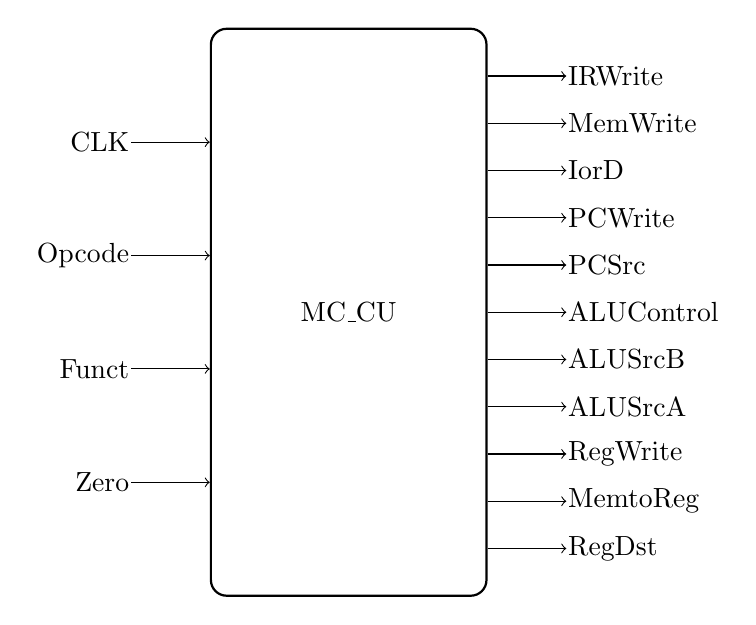
\begin{tikzpicture}
\draw node [draw,rectangle, minimum height=72mm, minimum width=35mm,rounded corners=2mm,thick](entity){};

\draw[->] ($ (entity.west)+(-10mm,21.6mm)$) -- ($ (entity.west) + (0mm,21.6mm)$);
\draw[anchor=east] node at ($ (entity.west)+(-9mm,21.6mm)$){ CLK };

\draw[->] ($ (entity.west)+(-10mm,7.2mm)$) -- ($ (entity.west) + (0mm,7.2mm)$);
\draw[anchor=east] node at ($ (entity.west)+(-9mm,7.2mm)$){ Opcode };

\draw[->] ($ (entity.west)+(-10mm,-7.2mm)$) -- ($ (entity.west) + (0mm,-7.2mm)$);
\draw[anchor=east] node at ($ (entity.west)+(-9mm,-7.2mm)$){ Funct };

\draw[->] ($ (entity.west)+(-10mm,-21.6mm)$) -- ($ (entity.west) + (0mm,-21.6mm)$);
\draw[anchor=east] node at ($ (entity.west)+(-9mm,-21.6mm)$){ Zero };


\draw[->] ($ (entity.east) + (0mm,30.0mm)$) -- ($ (entity.east) + (10mm,30.0mm)$);
\draw[anchor=west] node at ($ (entity.east) + (9mm,30.0mm)$){ IRWrite };

\draw[->] ($ (entity.east) + (0mm,24.0mm)$) -- ($ (entity.east) + (10mm,24.0mm)$);
\draw[anchor=west] node at ($ (entity.east) + (9mm,24.0mm)$){ MemWrite };

\draw[->] ($ (entity.east) + (0mm,18.0mm)$) -- ($ (entity.east) + (10mm,18.0mm)$);
\draw[anchor=west] node at ($ (entity.east) + (9mm,18.0mm)$){ IorD };

\draw[->] ($ (entity.east) + (0mm,12.0mm)$) -- ($ (entity.east) + (10mm,12.0mm)$);
\draw[anchor=west] node at ($ (entity.east) + (9mm,12.0mm)$){ PCWrite };

\draw[->] ($ (entity.east) + (0mm,6.0mm)$) -- ($ (entity.east) + (10mm,6.0mm)$);
\draw[anchor=west] node at ($ (entity.east) + (9mm,6.0mm)$){ PCSrc };

\draw[->] ($ (entity.east) + (0mm,0.0mm)$) -- ($ (entity.east) + (10mm,0.0mm)$);
\draw[anchor=west] node at ($ (entity.east) + (9mm,0.0mm)$){ ALUControl };

\draw[->] ($ (entity.east) + (0mm,-6.0mm)$) -- ($ (entity.east) + (10mm,-6.0mm)$);
\draw[anchor=west] node at ($ (entity.east) + (9mm,-6.0mm)$){ ALUSrcB };

\draw[->] ($ (entity.east) + (0mm,-12.0mm)$) -- ($ (entity.east) + (10mm,-12.0mm)$);
\draw[anchor=west] node at ($ (entity.east) + (9mm,-12.0mm)$){ ALUSrcA };

\draw[->] ($ (entity.east) + (0mm,-18.0mm)$) -- ($ (entity.east) + (10mm,-18.0mm)$);
\draw[anchor=west] node at ($ (entity.east) + (9mm,-18.0mm)$){ RegWrite };

\draw[->] ($ (entity.east) + (0mm,-24.0mm)$) -- ($ (entity.east) + (10mm,-24.0mm)$);
\draw[anchor=west] node at ($ (entity.east) + (9mm,-24.0mm)$){ MemtoReg };

\draw[->] ($ (entity.east) + (0mm,-30.0mm)$) -- ($ (entity.east) + (10mm,-30.0mm)$);
\draw[anchor=west] node at ($ (entity.east) + (9mm,-30.0mm)$){ RegDst };


\draw node at ($ (entity) - (0,0mm)$){ MC\_CU };

\end{tikzpicture}
\end{center}

Do not change the file ``MC\_CU.vhdl".\\

You will have to implement the following types of instructions:

%%selected_instruction_type_text

Before the execution of an instruction the instruction has to be fetched and decoded. This takes two clock cycles. During the fetch clock cycle the instruction is read from the current program counter value (PC) and is saved to the instruction register. Also during the fetch clock cycle the PC register is incremented by 4 using the ALU. The next clock cycle is used to decode the instruction in the control unit. %%beq_bne_decode_addition \\

The ``MC\_CU" entity shall control the multicycle processor depicted in Figure~1 to perform the following instructions:

\begin{table}[h!]
\centering
    \begin{tabular}{|c|c|c|c|c|} \hline \Tstrut
		instruction & opcode  & funct & type   \\ \hline \Tstrut
		%%selected_instruction_table_text
    \hline
    \end{tabular}
\end{table}

%%first_instruction_text \\

%%second_instruction_text \\

\begin{table}[h!]
\centering
    \begin{tabular}{|c|c|} \hline \Tstrut
		ALUControl & Function   \\ \hline \Tstrut
		%%ALUControl_table
    \hline
    \end{tabular}
    \caption{ALUControls}
    \label{tab:ALUControls}
\end{table}

To get a better understanding of the control signals, here is a description of each control
signal. Use Figure~1 to see how the control signals control the data paths.

\begin{itemize}

\item{IRWrite: When IRWrite is set to `1' then the instruction read from instruction memory gets written to the instruction register, at a rising edge of the CLK signal.}

\item{MemWrite: When MemWrite is set to `1' then the data memory input write data is written to the data memory input address, at a rising edge of the CLK signal.}

\item{IorD: Selects whether the data memory input address comes from the program counter register or from the ALU Result register.}

\item{PCWrite: When PCWrite is set to `1' then the program counter register is written, at a rising edge of the clock signal.}

\item{PCSrc: Selects whether the new program counter value shall come from the ALU, the ALU Result register or the jump address.}

\item{ALUControl: Selects the ALU operation the ALU performs on its two input values. The controls for the available operations are listed in Table~1.}

\item{ALUSrcB: Selects whether the ALU gets a value from the registers read data 2 output, from a constant value of 4, from the sign extended immediate value of the instruction or from the sign extended immediate value of the instruction shifted left by 2 bits.}

\item{ALUSrcA: Selects whether the ALU gets a value from the registers read data 1 output or from the program counter register.}

\item{RegWrite: When RegWrite is set to `1' then the registers write data input is written to the register specified by the write register input, at a rising edge of the clock signal.}

\item{MemtoReg: Selects whether the write data for the registers comes from data memory or from the ALU Result register.}

\item{RegDst: Selects whether the write register input for the registers comes from bits 20~--~16 of the instruction or from bits 15 -- 11 of the instruction.}

\end{itemize}

Consider which actions each part of the processor in Figure~1 has to take to fulfill the functions of the operations and set the control signals accordingly. This behavior has to be programmed in the attached file ``MC\_CU\_beh.vhdl".\\


To turn in your solution write an email to %%SUBMISSIONEMAIL with Subject ``Result Task %%TASKNR" and attach your behavior file ``MC\_CU\_beh.vhdl"


\vspace{0.7cm}
Good Luck and May the Force be with you.

\begin{landscape}
\begin{figure}[!h]
\vspace{-1cm}
\hspace{-1.8cm}
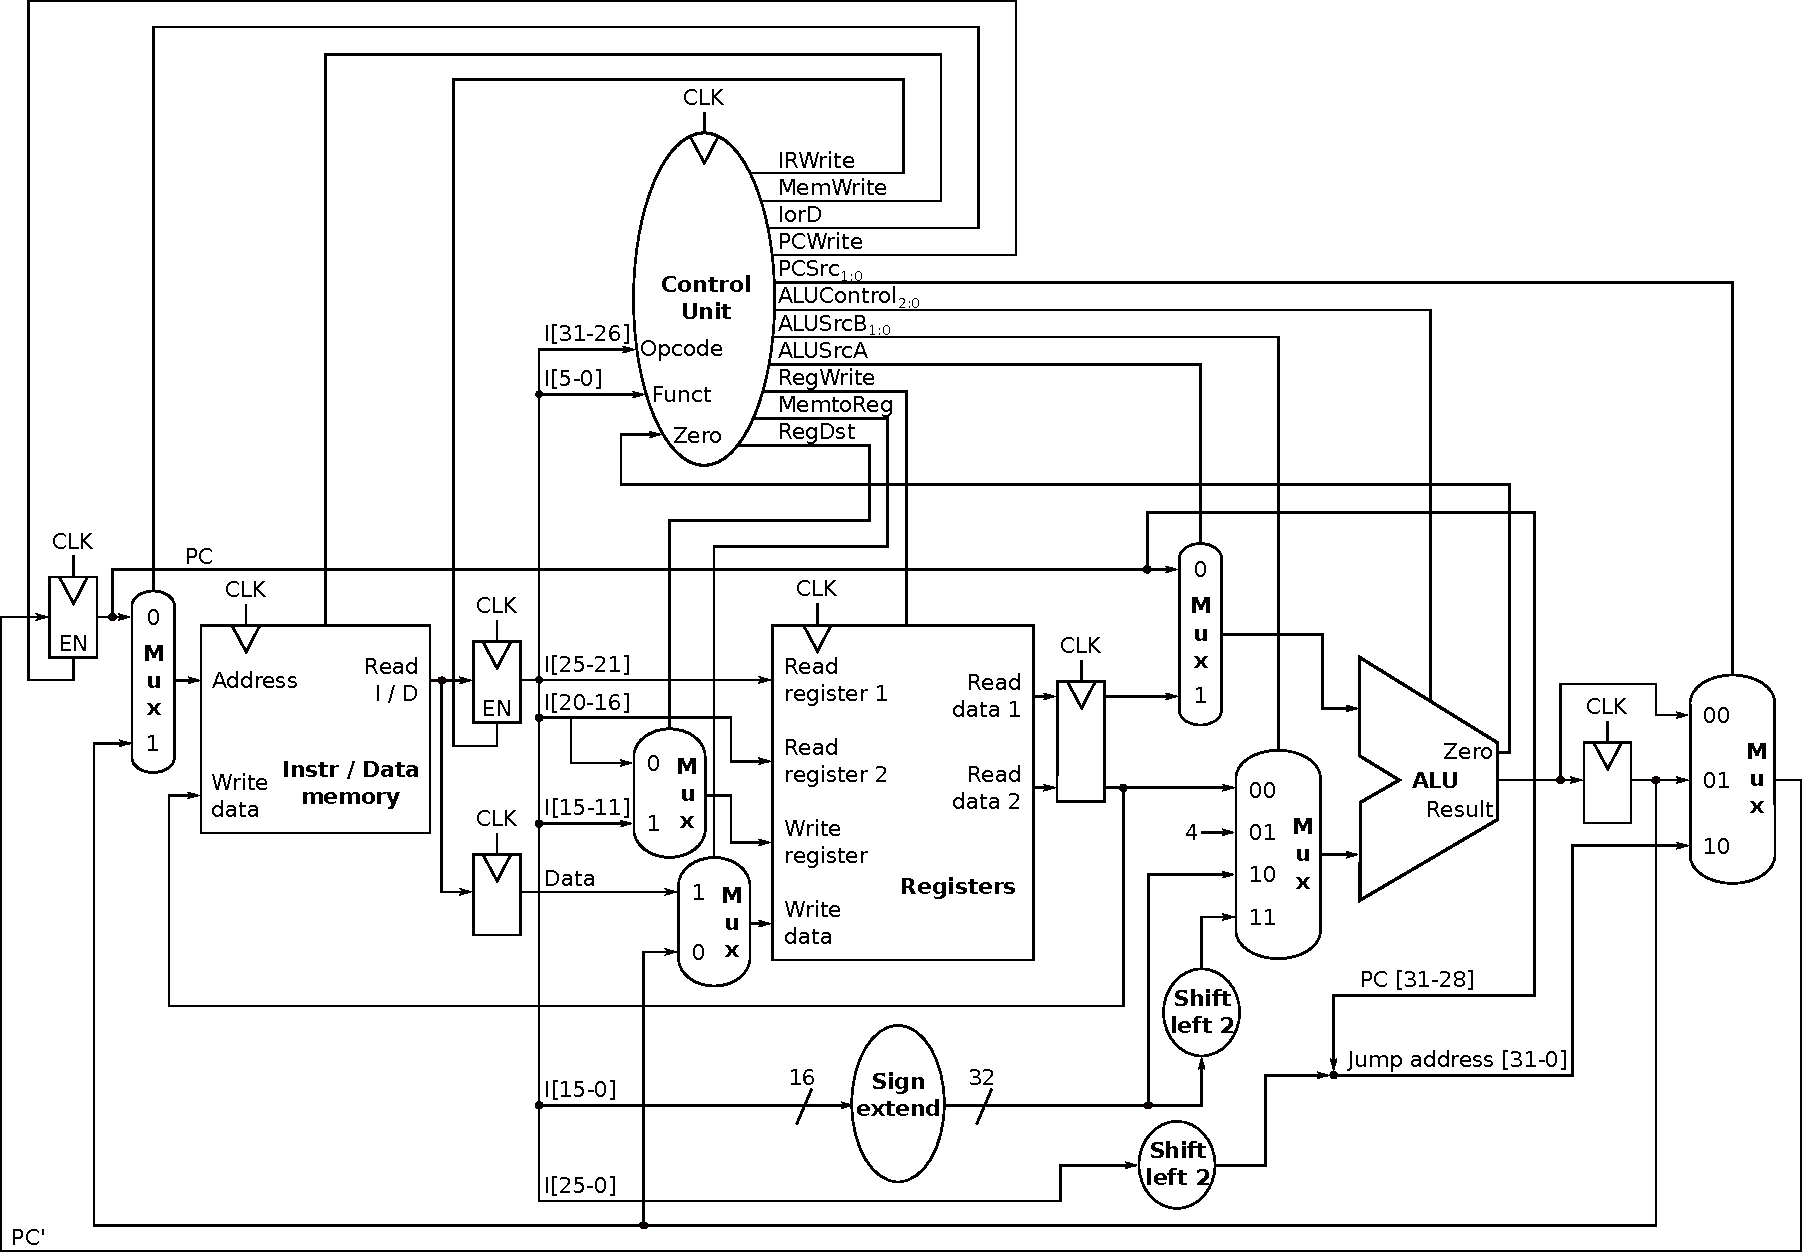
\includegraphics[width=25.5cm]{Multicycle_Processor_V_1_3}
\caption{Multicycle processor}
\label{fig:MulticycleProcessor}
\end{figure}
\end{landscape}

\end{document}